\chapter{Groundwave}

When transmitting from one radio to another the signal travel as electromagnetic waves, these waves can reach the receiver taking multiple paths. It could be a direct path from transmitter to receiver, or a reflected wave of a surface such as the ground this can be seen in \autoref{fig:directReflectedPath}. 

\begin{figure}[H]
\centering
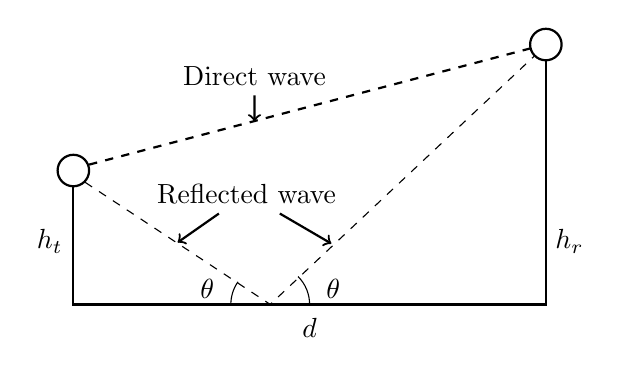
\begin{tikzpicture}[scale=0.1]

\node (v1) at (-30,-8) {};
\node (v2) at (30,8) {};

\draw[thick]  (v1) circle (2);
\draw[thick]  (v2) circle (2);

\draw[thick]  (-30,-10)  -- (-30,-25) -- (30,-25) --  (30,6) ;

\node at (-33,-17) {$h_t$};
\node at (33,-17) {$h_r$};
\node at (0,-28) {$d$};


\draw[dashed] (-28.5,-9.5) -- (-5,-25) -- (28.5,6.5);
\draw (-10,-25) arc (180:145:5);
\draw (-0,-25) arc (0:45:5);
\node at (-13,-23) {$\theta$};
\node at (3,-23) {$\theta$};
\draw[thick, dashed] (-28,-7.25) --  (28,7.5);
\node (v3) at (-8,-11) {Reflected wave};
\node (v6) at (-7,4) {Direct wave};
\node (v4) at (-18,-18) {};
\node (v5) at (4,-18) {};
\draw[->,thick]  (v3) edge (v4);
\draw[->,thick]  (v3) edge (v5);
\node (v7) at (-7,-3) {};
\draw[->,thick]  (v6) edge (v7);
\end{tikzpicture}

    

\caption{Direct and reflected path from transmitter to receiver}
\label{fig:directReflectedPath}
\end{figure}

This worksheet will focus on the paths close to the ground, and primarily on the surface wave component since the direct and reflected wave are described in further detail in ??. The ground acts both as a reflector and also as an absorber \citep{Bullington}. This means that a received wave can be contributed from three main factors. In 1947 Burlington wrote that \textit{"The principal effect of plane earth on the propagation of radio waves is indicated by the following equation"}\citep{Bullington}. The surface part comes from the grounds absorption of the electromagnetic wave, when the energy enters the ground it sets up ground currents. These currents are a representation of the imperfect reflection.    

\begin{equation}
E=E_0\left[\underbrace{1}_{direct}+\underbrace{R\text{e}^{j\Delta}}_{reflected}+\underbrace{(1-R)A\text{e}^{j\Delta}}_{surface}\right]
\end{equation}
\begin{where}
\va{E}{is the recieved field intensity}{$\frac{V}{m}$}
\va{$E_0$}{is the recieved field intensity in free space}{$\frac{V}{m}$}
\va{R}{is the reflection coefficient of the ground}{1}
\va{$\Delta$}{is the phase difference between direct and reflected wave}{rad}
\va{A}{is the surface-wave attenuation factor}{1}
\end{where}

The phase difference $\Delta$, is the difference in phase resulting only from the difference in length between the direct wave and the reflected wave, L, which can be found using geometry. The phase difference can be found as:
\begin{equation}
\Delta =2\pi \frac{L}{\lambda}
\end{equation}
\begin{where}
\va{L}{is the difference in length between the direct wave and the reflected wave}{m}
\va{$\lambda$}{is wavelenght}{m}
\end{where}

For a plane earth case meaning that there are no bumps or curvatures on the earth, its just plane then L is found as:
\begin{equation}
L=\sqrt{(h_t+h_r)^2+d^2}-d
\label{plane_earth}
\end{equation}
\begin{where}
\va{d}{is the distance between the transmitter and receiver}{m}
\va{$h_t$}{is the height of the transmitter}{m}
\va{$h_r$}{is the height of the receiver}{m}
\end{where}

For cases where the $d > 5(h_t+h_r)$ \autoref{plane_earth} can be approximated as \citep{Bullington}:
\begin{align}
L &=\frac{2h_th_r}{d} \\
\Delta &= 4\pi\frac{h_th_r}{d\lambda}
\end{align}

The reflection coeficient R is dependent on the incoming angle of the signal, $\theta$, as well as the electromagnetic properties of the ground, $\epsilon$ and $\sigma$. The relation can be written as\citep{Bullington}:

\begin{equation}
R=\frac{\sin(\theta)-z}{\sin(\theta)+z}
\end{equation}
\begin{where}
\va{z}{$\frac{\sqrt{\epsilon_0-\cos^2(\theta)}}{\epsilon_0}$ for vertical polerization}{1}
\va{z}{$\sqrt{\epsilon_0-\cos^2(\theta)}$ for horizontal polerization}{1}
\va{$\epsilon_0$}{is the complex relative permittivity  = $\epsilon-j60\sigma\lambda$}{1}
\va{$\epsilon$}{is the dielectric constant of the ground relative to unity
in free space}{1}
\va{$\sigma$}{is the conductivity of the ground in mhos per meter}{$\frac{mhos}{m}$}
\va{$\theta$}{is reflection angle}{rad}
\end{where}

By looking at this equation it can be seen that as $\theta$ goes towards 0, R goes towards -1. Which also implies that for sufficiently low receiver and transmitter, the direct and reflected wave is completely out of phase since $R\text{e}^{j\Delta} = -1$. This leaves only the surface wave part of the equation.

The surface wave attenuation factor can be approximated as\citep{Bullington}

\begin{equation}
A\approx\frac{-1}{1+j\frac{2\pi d}{\lambda}\left(\sin(\theta)+z\right)^2}
\end{equation}

This approximation holds for $A<0.1$, however for A approaching unity the phase approaches 180 degree \citep{Bullington}. 

When $\theta$ approaches zero only the surface wave component remain and it is thus sufficient to look at the magnitude of it \citep{Chong}
\begin{align}
|(1-R)A| &\approx \left|2 \frac{-1}{1+j\frac{2\pi d}{\lambda}\left(\sin(\theta)+z\right)^2} \right| \\
|(1-R)A| &\approx \frac{2}{\frac{2\pi d}{\lambda}z^2} \label{eq:surfaceApprox}
\end{align}

By introducing $h_0$, the minimum effective antenna height, as:
\begin{equation}
h_0=\left| \frac{\lambda}{2\pi z} \right|
\end{equation} 
\begin{where}
\va{$h_0$}{is the minimum effective antenna height}{m}
\end{where}

By utilizing this \autoref{eq:surfaceApprox}, can be written as:
\begin{equation}
|(1-R)A| \approx \frac{4 \pi h_0^2}{\lambda d}
\end{equation}

The received power can then be found using \citep{Chong}
\begin{align}
P_r&=P_0 \left(\frac{E}{E_0}\right)^2 \\
P_r&=P_tG_rG_t\frac{\lambda^2}{(4\pi )^2 d^2} \left(\frac{E}{E_0}\right)^2\\
P_r&=P_tG_rG_t\left(\frac{h_0}{d}\right)^4
\end{align}
\begin{where}
\va{$P_r$}{is the received power at the receiver antenna}{W}
\va{$P_0$}{is the predicted power by the free space model (see free space model worksheet)}{W}
\va{$P_t$}{is the transmitted power from the transmitter}{W}
\va{$G_r$}{is the gain of the receiver antenna}{1}
\va{$G_t$}{is the gain of the transmitter antenna}{1}
\end{where}





%\va{•}{•}{•}













